% !TEX root = ./main.tex

\subsection{Input file}

Now let's have a look at the input file.
A typical input file has a structure like:
\begin{verbatim}
Test                              (title)
md                                (calc)
s       n                         (ic,iio)
10.00000                          (alatt)
1       1       1                 (nsc)
1.00000   0.00000   0.00000       (avec)
0.00000   1.00000   0.00000
0.00000   0.00000   1.00000
0.00100   0.00000                 (cmass, press)
1                                 (ntype)
4       Ar      36.00000          (natom,nameat,atmass)
0.00000   0.00000   0.00000       (rat)
0.50000   0.50000   0.00000
0.00000   0.50000   0.50000
0.50000   0.00000   0.50000
40                                (rcut)
6       6       6                 (ncell)
1000    100     10                (nstep,ntcheck,ntimes)
0.00000   0.00100   200.00000     (temp,ttol,dt)
\end{verbatim}

This input file investigates $4$ \ce{Ar} atoms in a conventional FCC unit cell,
\ce{Ar}'s atomic mass is selected to be \SI{36.0}{\atomicmassunit},
see Fig. \ref{fig:fcc1} for its crystal structure.
The \texttt{calc} flag specifies calculation type, including \texttt{md},
\texttt{cd}, \texttt{nd}, \texttt{sd}, \texttt{mm}, \texttt{cm}, \texttt{nm}, and \texttt{sm}, as we mentioned in the beginning of Sec. \ref{sec:mdc}.
\texttt{nsc} means the number of cells consisting a supercell in each direction of a 3D space.
\texttt{cmass} is $W$ as mentioned, in atomic unit. But it does not seem to have functions in Andersen's \texttt{md}.
The \texttt{press} is external pressure $P$, but in unit of \si{\mega\bar}.
\texttt{rcut} is the cut-off radius for this molecular dynamics, beyond which interatomic interactions are ignored, so the sphere defined by
\texttt{rcut} must be contained inside the stack of supercells, which is $7=2\times 3+1$ supercells in each direction (implemented in \texttt{CRSTL} subroutine). We usually choose numbers for \texttt{ncell}, to make
\texttt{alatt} times \texttt{ncell} greatly larger than \texttt{rcut}, for the supercells are
oscillating their volume in this molecular dynamics.
If not, the atoms may drift away, and the dynamical energies might not conserve.
Here we have $4=4 \times 1^3$ atoms inside one supercell.
Make sure that \texttt{ntcheck} times \texttt{ntimes} is greater than
\texttt{nstep}, the total number of time steps.
And \texttt{dt} times \texttt{nstep} is the total simulation time in Rydberg unit, which is
\SI{4.8378e-17}{\second} per unit time. \texttt{dt} times \texttt{nstep} is the total simulation time,
they are labeled on the upper horizontal axis in all my plots.

\begin{figure}[H]
	\begin{minipage}[t]{0.48\textwidth}
		\centering
		\input{Tikz/FCC1}
		\caption{A conventional FCC unit cell of \ce{Ar}.}
		\label{fig:fcc1}
	\end{minipage}
	\hfill
	\begin {minipage}[t]{0.48\textwidth}
	\centering
	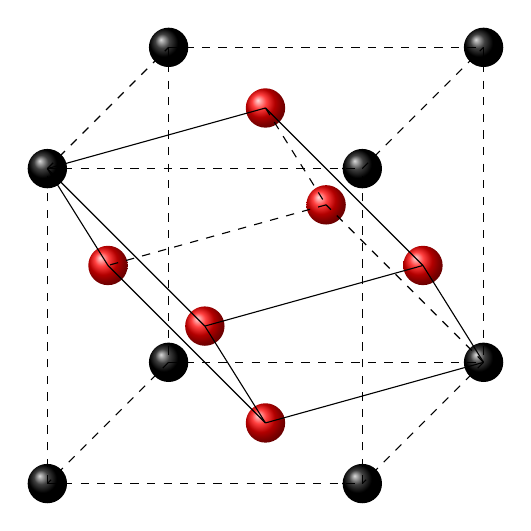
\begin{tikzpicture}
 %points on cube
 \coordinate (A) at (0,0,0);
 \coordinate (B) at (0,0,4);
 \coordinate (D) at (0,4,0);
 \coordinate (C) at (0,4,4);
 \coordinate (E) at (4,0,0);
 \coordinate (F) at (4,0,4);
 \coordinate (H) at (4,4,0);
 \coordinate (G) at (4,4,4);

 %center of faces
 \coordinate (I) at (0,2,2); %center of face ABCD
 \coordinate (J) at (4,2,2); %center of face EFGH
 \coordinate (K) at (2,4,2); %center of face DCGH
 \coordinate (L) at (2,0,2); %center of face ABFE
 \coordinate (M) at (2,2,4); %center of face CBGF
 \coordinate (N) at (2,2,0); %center of face DAEH

 %place non-atom cube corners
 \shade [ball color= black] (A) circle (0.25cm);
 \shade [ball color= black] (C) circle (0.25cm);
 \shade [ball color= black] (F) circle (0.25cm);
 \shade [ball color= black] (H) circle (0.25cm);
 \shade [ball color= black] (B) circle (0.25cm);
 \shade [ball color= black] (D) circle (0.25cm);
 \shade [ball color= black] (E) circle (0.25cm);
 \shade [ball color= black] (G) circle (0.25cm);

 %draw the center of each face
 \shade [ball color= red] (I) circle (0.25cm);
 \shade [ball color= red] (J) circle (0.25cm);
 \shade [ball color= red] (K) circle (0.25cm);
 \shade [ball color= red] (L) circle (0.25cm);
 \shade [ball color= red] (M) circle (0.25cm);
 \shade [ball color= red] (N) circle (0.25cm);

 %draw cube
 \draw [dashed] (A) -- (B);
 \draw [dashed] (B) -- (C);
 \draw [dashed] (C) -- (D);
 \draw [dashed] (D) -- (A);
 \draw [dashed] (E) -- (F);
 \draw [dashed] (F) -- (G);
 \draw [dashed] (G) -- (H);
 \draw [dashed] (H) -- (E);
 \draw [dashed] (A) -- (E);
 \draw [dashed] (B) -- (F);
 \draw [dashed] (C) -- (G);
 \draw [dashed] (D) -- (H);
 
 %draw unit cell
 \draw (E) -- (L);
 \draw (E) -- (J);
 \draw [dashed] (E) -- (N);
 \draw (J) -- (M);
 \draw (L) -- (M);
 \draw (J) -- (K);
 \draw [dashed] (K) -- (N);
 \draw (K) -- (C);
 \draw (M) -- (C);
 \draw (L) -- (I);
 \draw [dashed] (N) -- (I);
 \draw (C) -- (I);
\end{tikzpicture}

	\caption{A primitive FCC unit cell of \ce{Ar}, with
		vertices filled in red.}
	\label{fig:fcc3}
	\end{minipage}
\end{figure}

Now we are going to play with Wentzcovitch's molecular dynamics, to see what the
actual ``dynamics'' is. Suppose we have a file named \texttt{inp1}, listed below.
We will use this file as an example for comparison.
\begin{verbatim}
Test                              (title)
nd                                (calc)
s       n                         (ic,iio)
11.00000                          (alatt)
1       1       1                 (nsc)
1.00000   0.00000   0.00000       (avec)
0.00000   1.00000   0.00000
0.00000   0.00000   1.00000
0.00100   0.00000                 (cmass, press)
1                                 (ntype)
4       Ar      36.00000          (natom,nameat,atmass)
0.00000   0.00000   0.00000       (rat)
0.50000   0.50000   0.00000
0.00000   0.50000   0.50000
0.50000   0.00000   0.50000
40                                (rcut)
6       6       6                 (ncell)
2000    100     10                (nstep,ntcheck,ntimes)
0.00000   0.00100   75.00000      (temp,ttol,dt)
\end{verbatim}

\newpage
Here we are going to use \texttt{dt} $= 75$ in Rydberg unit and $2000$ time steps. This is because, different \texttt{dt} could result in different decaying rates.
We run this file with $4$ different \texttt{dt}, $150$, $200$, $300$ and $400$
Rydberg unit respectively.
But totally simulate both $600000$ in Rydberg time unit. From Fig. \ref{fig:inp1:mini:subfig:b} we can see a noticeable
decreasing in total energy, but for Fig. \ref{fig:inp1:mini:subfig:a} this is less distinguishable. For Fig. \ref{fig:inp1:mini:subfig:c} and Fig. \ref{fig:inp1:mini:subfig:d}
this situation is even worse, the total energy decays even faster, showing an unstable dynamics. This can be understood since in
Beeman algorithm we assume the length of each time step $h$ is a small quantity (see Eq. \eqref{eq:beeman}),
for we are using Taylor expansion implicitly. So when $h$ is too large, numerical errors
could be apparent.

\begin{figure}[h]
	\centering
	\begin{minipage}[t]{0.48\textwidth}
		\centering
		\includegraphics[width=\linewidth]{4000_150_100_4}
		\subcaption{$4000$ time steps, with each time step to be $150$ Rydberg unit.}
		\label{fig:inp1:mini:subfig:a}   %% label for first subfigure 
	\end{minipage}
	\hfill
	\begin{minipage}[t]{0.48\textwidth}
		\centering
		\includegraphics[width=\linewidth]{3000_200_100_9}
		\subcaption{$3000$ time steps, with each time step to be $200$ Rydberg unit.}
		\label{fig:inp1:mini:subfig:b}   %% label for second subfigure 
	\end{minipage}
	\begin{minipage}[t]{0.48\textwidth}
		\centering
		\includegraphics[width=\linewidth]{2000_300_100_0}
		\subcaption{$2000$ time steps, with each time step to be $300$ Rydberg unit.}
		\label{fig:inp1:mini:subfig:c}   %% label for third subfigure 
	\end{minipage}
	\hfill
	\begin{minipage}[t]{0.48\textwidth}
		\centering
		\includegraphics[width=\linewidth]{1500_400_100_2}
		\subcaption{$1500$ time steps, with each time step to be $400$ Rydberg unit.}
		\label{fig:inp1:mini:subfig:d}   %% label for fourth subfigure 
	\end{minipage}
	\caption{Wentzcovitch's \texttt{nd} for a conventional FCC cell of \ce{Ar} at \SI{0}{\kelvin} with $4$ different \texttt{dt} but the same total simulation time. Here fictitious mass $W$ is $0.001$.}
	\label{fig:inp1}   %% label for entire figure 
\end{figure}

So for easier observation,
in later discussion, \texttt{dt} $= 75$ in Rydberg unit and $2000$ time steps are chosen.
The results are plotted in Fig. \ref{fig:inp1run} for references.

\begin{figure}[h]
	\begin{minipage}[t]{0.48\textwidth}
		\centering
		\includegraphics[width=\linewidth]{2000_75_100_8}
		\subcaption{Energies of the conventional cell and atoms versus time.}
		\label{fig:inp1run:mini:subfig:a}   %% label for first subfigure 
	\end{minipage}
	\hfill
	\begin{minipage}[t]{0.48\textwidth}
		\centering
		\includegraphics[width=\linewidth]{2000_75_100_2_avec}
		\subcaption{Cell vectors oscillation versus time, $a=b=c$ for this is a cubic crystal.}
		\label{fig:inp1run:mini:subfig:b}   %% label for second subfigure 
	\end{minipage}
	\caption{Wentzcovitch's \texttt{nd} for a conventional FCC cell of \ce{Ar} at \SI{0}{\kelvin}, with \texttt{dt} $=75$, $2000$ time steps, $W = 0.001$.}
	\label{fig:inp1run}   %% label for entire figure 
\end{figure}

From Fig. \ref{fig:inp1run:mini:subfig:b} we can approximately assume that the equilibrium
lattice parameter is around \SI{9.9}{\bohr}, where vibration happens back and forth.
But the code also provides a \texttt{nm} algorithm by adding a damping mechanism
to let us compute energy-minimized structure quickly. So we keep the fictitious mass fixed,
and then run the structural optimization algorithm. The stabilized structure also has a
lattice parameter around \SI{9.9}{\bohr}, which strengthen the credibility of our MD result.
See Fig. \ref{fig:inp5} for references.

\begin{figure}[H]
	\begin{minipage}[t]{0.48\textwidth}
		\centering
		\includegraphics[width=\linewidth]{100_500_2010_9}
		\subcaption{Energies for structure minimization versus time.}
		\label{fig:inp5:mini:subfig:a}   %% label for first subfigure 
	\end{minipage}
	\hfill
	\begin{minipage}[t]{0.48\textwidth}
		\centering
		\includegraphics[width=\linewidth]{100_500_2010_3_avec}
		\subcaption{Lattice parameters versus time, the final result is around \SI{9.9}{\bohr}.
			We can see inflections points on the curve, that's where the velocity changes sign and then forced to be $0$.}
		\label{fig:inp5:mini:subfig:b}   %% label for second subfigure 
	\end{minipage}
	\caption{Wentzcovitch's structural optimization algorithm \texttt{nm} for a conventional FCC cell of \ce{Ar}, with \texttt{dt} $=500$, $100$ time steps, and $W = 0.001$.}
	\label{fig:inp5}   %% label for entire figure 
\end{figure}

By far we only investigated the conventional cell of FCC \ce{Ar}.
Now let's come to the primitive cell. Inside,
there is only $1$ \ce{Ar} atom in the cell, shown in Fig. \ref{fig:fcc3}. Thus the cell size decreases to $\frac{ 1 }{ 4 }$ of the original one (defined in \texttt{inp1}).
Other parameters are the same as \texttt{inp1}.
The results are shown in Fig. \ref{fig:inp3run}.

\begin{figure}[H]
	\begin{minipage}[t]{0.48\textwidth}
		\centering
		\includegraphics[width=\linewidth]{2000_75_100_0}
		\subcaption{Energies of the primitive cell and atoms versus time.}
		\label{fig:inp3run:mini:subfig:a}   %% label for first subfigure 
	\end{minipage}
	\hfill
	\begin{minipage}[t]{0.48\textwidth}
		\centering
		\includegraphics[width=\linewidth]{2000_75_100_5_avec}
		\subcaption{Cell vectors oscillation versus time.}
		\label{fig:inp3run:mini:subfig:b}   %% label for second subfigure 
	\end{minipage}
	\caption{Wentzcovitch's \texttt{nd} for a primitive FCC cell of \ce{Ar} at \SI{0}{\kelvin}, with \texttt{dt} $=75$, $2000$ time steps, $W = 0.001$.}
	\label{fig:inp3run}   %% label for entire figure 
\end{figure}

\begin{figure}[h]
	\centering
	\begin{minipage}[t]{.48\linewidth}
		\centering
		\includegraphics[width=\linewidth]{2000_75_100_3}
		\subcaption{Energies of the primitive cell and atoms versus time.}
		\label{fig:inp4:a}
	\end{minipage}%
	\hfill
	\begin{minipage}[t]{.48\linewidth}
		\centering
		\includegraphics[width=\linewidth]{2000_75_100_0_avec}
		\subcaption{Cell vectors oscillation versus time.}
		\label{fig:inp4:b}
	\end{minipage}
	\caption{
		Wentzcovitch's \texttt{nd} for a primitive FCC cell of \ce{Ar} at \SI{0}{\kelvin}, with \texttt{dt} $=75$, $2000$ time steps, $W = 0.004$.}
	\label{fig:inp4}
\end{figure}

However, in comparison with Fig. \ref{fig:inp1run},
the oscillation frequencies of energies and lattice parameters
both increase by a factor of $2$, which is not astonishing because from
\eqref{eq:hdd} we know that
\begin{equation}
	\omega \propto \sqrt{
		\frac{ B }{ W V }
	},
\end{equation}
where $B$ is the bulk modulus, a fixed quantity for every material. So to make this MD
have the same frequency as \texttt{inp1}, we need to adjust the fictitious mass $W$ to be
four times of the original one, i.e., $0.004$.
Now the result, shown in Fig. \ref{fig:inp4}, is the same as Fig. \ref{fig:inp1run}. So we find a powerful tool! Whenever the cell volume has changed, we can always
adjust $W$ to recover the original frequencies. We will talk about this a little bit later.

\begin{figure}[h]
	\centering
	\begin{minipage}[t]{0.48\textwidth}
		\centering
		\includegraphics[width=\linewidth]{Andersen_2000_75_100_5}
		\subcaption{Every atom sits in exactly their equilibrium coordinates.}
		\label{fig:andersen0:mini:subfig:a}   %% label for first subfigure 
	\end{minipage}
	\hfill
	\begin{minipage}[t]{0.48\textwidth}
		\centering
		\includegraphics[width=\linewidth]{Andersen_2000_75_100_3}
		\subcaption{One of the $4$ atoms shifts a little from its equilibrium coordinate.}
		\label{fig:andersen0:mini:subfig:b}   %% label for second subfigure 
	\end{minipage}
	\caption{Andersen's \texttt{md} for a conventional FCC cell of \ce{Ar} at \SI{0}{\kelvin}, with
		\texttt{dt} $=75$, $2000$ time steps.}
	\label{fig:andersen0}   %% label for entire figure 
\end{figure}

Now we run the code using Andersen's molecular dynamics \texttt{md}, to find the oscillation frequency of atoms. This is done at \SI{0}{\kelvin}, so we have to shift the atoms a little from their equilibrium
positions, or else we will not observe any oscillation phenomenon, like in Fig. \ref{fig:andersen0:mini:subfig:a}.
For instance, in Fig. \ref{fig:andersen0:mini:subfig:b} we can roughly assume that
one period of this oscillation is $200$ time steps, with each $75$ Rydberg unit.

\begin{figure}[H]
	\centering
	\begin{minipage}[t]{.48\linewidth}
		\centering
		\includegraphics[width=\linewidth]{2000+75+100-3}
		\subcaption{Energies of the primitive cell and atoms versus time.}
		\label{fig:adjust:a}
	\end{minipage}%
	\hfill
	\begin{minipage}[t]{.48\linewidth}
		\centering
		\includegraphics[width=\linewidth]{2000+75+100-9avec}
		\subcaption{Cell vectors oscillation versus time.}
		\label{fig:adjust:b}
	\end{minipage}
	\caption{Wentzcovitch's \texttt{nd} for a conventional FCC cell of \ce{Ar} at \SI{0}{\kelvin},
		with \texttt{dt} $= 75$, $2000$ time steps, $W = 0.0026$.}
	\label{fig:adjust}
\end{figure}

Then we do Wentzcovitch's MD, by adjusting fictitious mass $W$, we let the oscillation
period of cell vectors to be the same as that of the atoms' from last step, i.e., $200$ time
steps. Here a good value is $W = $ \SI{0.0026}{\atomicmassunit}. See Fig. \ref{fig:adjust} for references. Why we need to do this? Because we have two integrators for this molecular dynamics,
one is for atoms and one is for cell, if we synchronize their oscillation frequencies, then
integrator with larger period need not to wait for the other one. This will save computational
time.

\begin{figure}[H]
	\centering
	\begin{minipage}[t]{.48\linewidth}
		\centering
		\includegraphics[width=\linewidth]{32_atom_2000+75+100-3}
		\subcaption{Energies of the primitive cell and atoms versus time.}
		\label{fig:32atom:a}
	\end{minipage}%
	\hfill
	\begin{minipage}[t]{.48\linewidth}
		\centering
		\includegraphics[width=\linewidth]{32_atom_2000+75+100-5avec}
		\subcaption{Cell vectors oscillation versus time.}
		\label{fig:32atom:b}
	\end{minipage}
	\caption{Wentzcovitch's \texttt{nd} for $32$ \ce{Ar} atoms at \SI{0}{\kelvin},
		with \texttt{dt} $= 75$, $2000$ time steps, $W = 0.000325$.}
	\label{fig:32atom}
\end{figure}

After this step, we can extend this MD with more atoms (larger supercells), like a $32$-atom-supercell.
Now a supercell is constructed by $8 = 2 \times 2 \times 2$ unit cells, thus its volume has
increased to $8$ times of the last one. But if we want to keep the cell oscillation and atomic
oscillation synchronized, we need to reduce $W$ to its $\frac{ 1 }{ 8 }$, i.e., $0.000325$. See
Fig. \ref{fig:32atom} for references.

This code now has been implemented in \textsc{Quantum ESPRESSO}, the \texttt{vc-relax}
calculation. For \texttt{cell\_dynamics} flag, option \texttt{damp-w} uses \texttt{nm} introduced above, \texttt{none} uses \texttt{mm}, and \texttt{damp-pr} corresponds to \texttt{cm}.
For \texttt{vc-md} flag, option \texttt{w} uses \texttt{nd}, \texttt{none} uses \texttt{md}, and \texttt{pr} uses \texttt{cd}.
